\subsection{General domain: KBP37 based distantly supervised dataset} 
As it was mentioned before KBP37 dataset was adapted from the MIML-RE dataset from 
\cite{angeli2014combining}. In order to evaluate Distant Supervision in general domain, this dataset was 
chosen, as authors of \cite{angeli2014combining} made publicly available the set of relation 
pairs that were used for the creation of the dataset. They used 2010 and 2013 TAC KBP \footnote{\url{https://www.ldc.upenn.edu/collaborations/current-projects/tac-kbp}} documents as a source of relations. 
For creating the supervised dataset they utilised Amazon Mechanical Turk \footnote{\url{https://www.mturk.com/mturk/welcome}} for labelling examples that they got after aligning entity pairs to 
sentences from 2013 Wikipedia dump. They annotated 23725 examples, that were transformed to 
KBP37 dataset by \cite{DBLP:journals/corr/ZhangW15a}.

A closer investigation of the entity pairs from TAC KBP showed that the quality of them is 
not high enough. For example, they could contain only one letter as a name or just a word ''president'' as an entity 
for ''org:top-members/employees'' relation.
Thus as a Knowledge Base for Distant Supervision experiments both relational pairs from MIML-RE 
\footnote{\url{https://nlp.stanford.edu/software/mimlre.shtml}}, i.e. from TAC KBP, and Wikidata 
\footnote{https://query.wikidata.org/} were used. Wikidata returned fewer pairs 
corresponding to required relations, but they are more precise. Entity pairs from Wikidata were 
queried through the query interface for each of the corresponding relations.  
The amount of entity pairs for each of the relation types varies a lot - from less than 1000 to more than 
50000. For creating the ''Other'' class were chosen ''per:religion'', ''per:children'', ''org:political/religious-affiliation'' 
entity pairs. In order to minimise noise effect of not accurate entity pairs from TAC KBP, 
the entity pairs containing one letter entities or names consisting only of capital letters with dots were filtered out and not used.

For raw text corpus the NewYork 
Times archive \footnote{\url{https://catalog.ldc.upenn.edu/ldc2008t19}} was taken.
According to the idea of the 
Distant Supervision an alignment of entity pairs from a Knowledge Base to the text should be performed. This was done by the 
simple method of string matching. It means that entities' names were simply searched 
in the textual corpus. If sentence included two entities that are related according to the Knowledge Base that would give an example
for the corresponding relation.
In order to implement the lookup of the words in a large volume of textual data, Whoosh, a python library for 
indexing the text, was used \footnote{\url{https://whoosh.readthedocs.io/en/latest/}}. It allows to index 
each sentence of the text as a separate entry and then make a request to search for two 
entities' names and returns all the entries containing them. So, raw textual data 
from NYT corpora was split into sentences with NLTK library, indexed by 
Whoosh and then aligned with the set of entity pairs from the Knowledge Base. If all 
of the aligned sentences are taken, it would lead to a highly unbalanced, both by the amount of 
examples per relational class and the amount of examples per entity pair, and really huge dataset. That is why 
only 5 examples per entity pair were taken and the maximal amount of sentences in relational class 
was set to 3000. This resulted in a dataset with the overall amount of 75913 sentences. And even this dataset is 
already almost tree times more than the supervised dataset for the same relational classes and it was obtained 
completely automatically. It proves the point, that the amount of distantly supervised training data can be 
made as large as needed without any additional effort.

Apart from simple training on the distantly supervised data, several experiments for quality 
improvement were held: 
\begin{itemize}
  \item Applying Multiple Instance Learning. As it was explained in Subsection \ref{subs:mil}, training 
  examples for this setup are bags containing at least one correctly labeled sentence. Thus sentences 
  were grouped based on the entity pair they contain and each of this bags was labeled as 
  a relation, that this entity pair has in the Knowledge Base.
  \item Mixing supervised data. It was mentioned in \cite{riedel2010modeling} that distantly 
  supervised data introduces noise, but it was decided to check how adding existing 
  supervised data into the distant dataset would affect the training results.
  \item Using transfer learning. Generally, it might be a good idea to train the model on 
  existing supervised data and then continue tuning it with more and more distantly supervised data to get better results.
\end{itemize}

\subsection{Results}
\label{subs:gen-dist-res}
The results of training the network in various ways with distantly supervised data can be seen
in the Table \ref{tab:dist-gen-res}. For comparison, the supervised training result was also included in the 
table.

\begin{table}
  \begin{center}
 \begin{tabular}{ | c | c | c | c | }
    \hline
    Experiment & P & R & F1 \\ \hline
    Supervised training & \textbf{67.74} & 57.88 & \textbf{61.26} \\ \hline
    Distantly supervised training & 50.71 & 45.24 & 43.81 \\ \hline
    Distantly supervised + MIL & 51.82 & 46.61 & 45.40 \\ \hline
    Distantly supervised + supervised data & 57.64 & 57.84 & 55.03 \\ \hline
    Distantly supervised + supervised data + MIL & 60.25 & \textbf{58.24} & 56.93 \\ \hline
    Transfer from supervised & 48.93 & 44.14 & 42.73 \\ \hline
    Transfer from supervised + MIL & 51.13 & 44.92 & 44.58 \\ \hline
    \end{tabular}
\caption[General domain, Distant Supervision experiments results]{Precision, Recall and F1-scores for distantly supervised training evaluation.}
\label{tab:dist-gen-res}
\end{center}
\end{table}

The first conclusion that can be made - training without manually labeled data can be performed and 
it will achieve definitely higher results than random assignment (with the amount of classes 37 
F1-score for random assignment would be around 0.2\%). Thus it was successfully proven, that 
having publicly available Knowledge Base with required relation types and a large amount of textual data 
training set for a neural network solving the task of Relation Extraction can be constructed automatically. In
the context of the task to continuously extract new knowledge from newly published texts, this approach is 
more appealing than manual extraction. Supervised training might give better results but it still 
requires the manually curated creation of training dataset, that is most of the times not possible and also 
should be repeated for any new relational class. Also, in real-world application, while validating the 
results for including into a Knowledge Base not only the top score answer might be considered. Thus, 
if only top one considered as an answer ratio of correct answers is 42.99\%. If top three answers 
are considered for checking, then already 68.14\% will be recognised correctly. Further addition does 
not change the result so much - with top five the percentage of correct answers is 79.58\%.

The second point is a definite positive effect of Multiple Instance Learning. Every time when Multiple Instance Learning was applied the previous result 
was improving by approximately two percents. Good point also that not only Precision or 
Recall alone is improved, but both simultaneously. It can be concluded, that exploration of further more complex 
methods for noise reduction in the distantly supervised data will significantly improve the score. 

The results of transfer learning experiment were disappointing, it performs even worse than 
simple distantly supervised training. It might be explained by different directions that datasets
are trying to lead the network - scopes of syntactic constructions in supervised dataset and in 
distantly supervised dataset might differ a lot. Thus pre-training with supervised data leads to a worse starting point for 
distantly supervised training than a random one.

As it was expected, mixing in existing supervised data improved drastically distantly 
supervised training. And also as expected, it gives a worse result than pure supervised training. But it should be 
pointed out that with Multiple Instance Learning together with mixed dataset setup, it was possible to reach higher Recall than for supervised 
training. This means that distantly supervised data helps the model to become more general, be 
less biased by the provided supervised dataset. It again might be a very good sign for live models, 
that are supposed to retrieve more and more new knowledge from new textual data, because
it is never possible to provide the needed amount of new labeled training data manually. 

\subsection{Interpretation}
\paragraph{Distantly and manually supervised datasets}
It is important, that manually supervised training and testing datasets are tightly coupled and they will have common 
context and common biases. Thus, evaluating distantly supervised model with existing testing
dataset might be not objective. There exist other ways to evaluate the results of Distant Supervision, for example, 
performed in \cite{Mintz:2009:DSR:1690219.1690287}, but they would not show a realistic comparison to the 
supervised results. Moreover, evaluation with supervised testing dataset allows having a fresh look at the 
quality of the supervised data. It might not be absolutely accurate, especially when the number of examples
is large. And the worst aspect is that the supervised training will cause bias to specific kind of mistakes (as they 
will be both in training and testing set).

Overall, if there exist a hypothetical full set of all possible syntactic constructions for describing a specific relation, 
supervised dataset would be some (most of the times not very big) subset of it and of course, 
it might contain errors of labelling, that both training and testing sets would share. On the 
other hand, distantly supervised dataset would be slightly different subset of the whole set, that 
might be spread more and more - thus evaluation with initial supervised testing set would be less 
and less objective, because some constructions that are not there would be recognised by the 
price of forgetting constructions from the supervised dataset. In general, this idea is reflected in the Figure \ref{fig:dist-superv-knowledge}.

\begin{figure}[H]
\centering
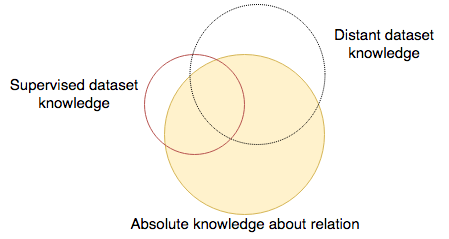
\includegraphics[width=250px]{chapter4_experiments/images/dist-superv-knowledge.png}
\caption[Relation of supervised and distantly supervised knowledge]{Concept of knowledge about a specific relation contained in supervised and distantly supervised datasets.}
\label{fig:dist-superv-knowledge}
\end{figure}

It seemed quite logical to suggest, that in order to have more basement for such conclusions one should look into the ratio of correctly
recognised examples for manually supervised and distantly supervised networks. The result of this investigation is depicted in the 
Figure \ref{fig:uniq-correct}. It can be seen, that for some of the relations manually supervised network will recognise much more 
constructions, but there are still relations for which distantly supervised network finds more constructions. Overall, a number of 
examples recognised only by the distantly supervised network is quite sensible. It can be concluded that the information contained 
in the distantly supervised dataset is useful and quite different from the one in the manually labeled dataset. Thus, the main 
goal when working with distantly supervised dataset is to get rid of the noise that lowers the precision of recognition.

\begin{figure}[H]
\centering
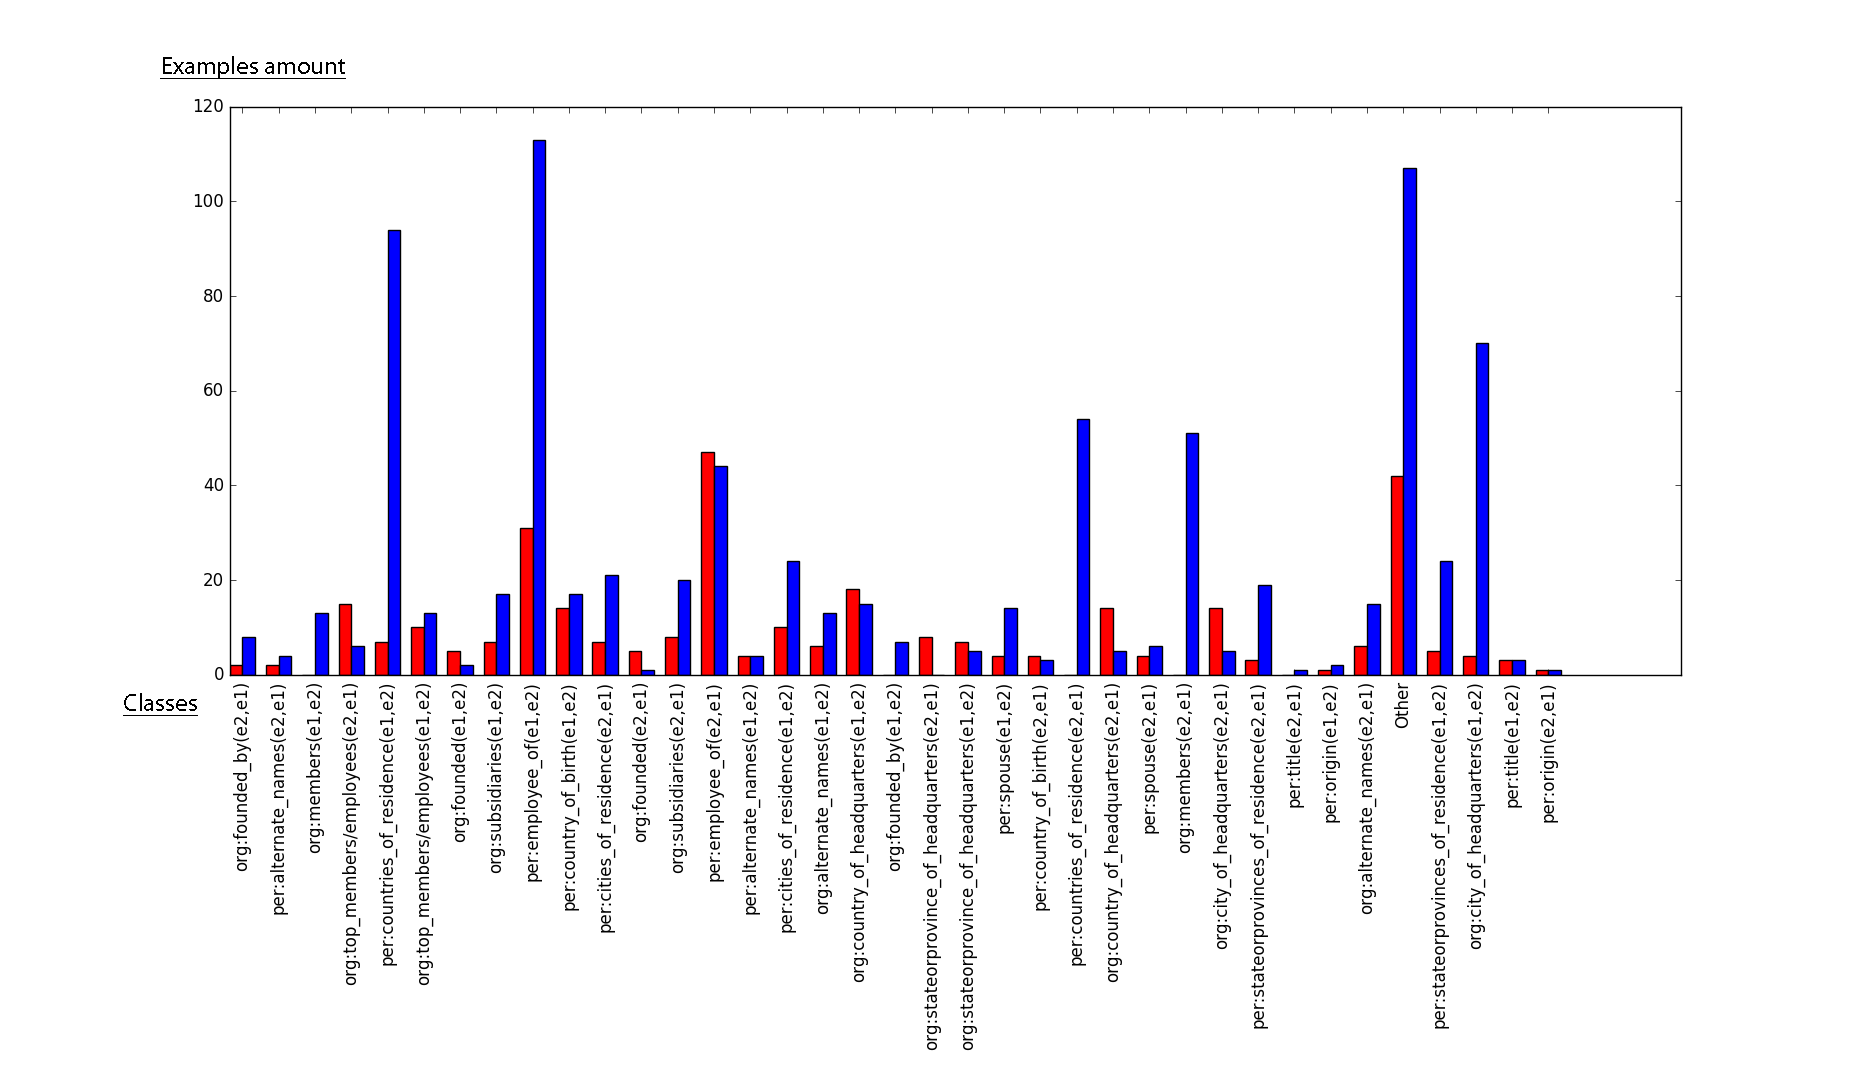
\includegraphics[width=\linewidth]{chapter4_experiments/images/uniq-correct.png}
\caption[Relation between correct answers for manually and distantly supervised training]{Blue bars show amount of testing examples that were recognised correctly by manually supervised network, but were not recognised by distantly supervised one. Red bars show the same amount for distantly supervised network.}
\label{fig:uniq-correct}
\end{figure}

\paragraph{Length of the examples}
\label{par:ex-length}
Of course one more very important aspect of relation recognition in a sentence is the length of the sentence and the distance
between the entities in it. The dependency can be seen in the Figure \ref{fig:dist-depend}. Spikes around the large values of length and  
distance are not representative, as the number of the examples there much smaller (3-5 sentences). But the overall the tendency 
is clearly seen - with the enlargement of the length or distance a number of errors grows and a number of right answers drops.
Any distantly supervised dataset will always be characterised by longer sentences on average, so this aspect should be taken into 
account when the dataset is constructed. For example, sentences longer than some limit can be simply not included in the 
final set of training examples.

\begin{figure}
\centering
\subfigure[Sentence length dependency]{
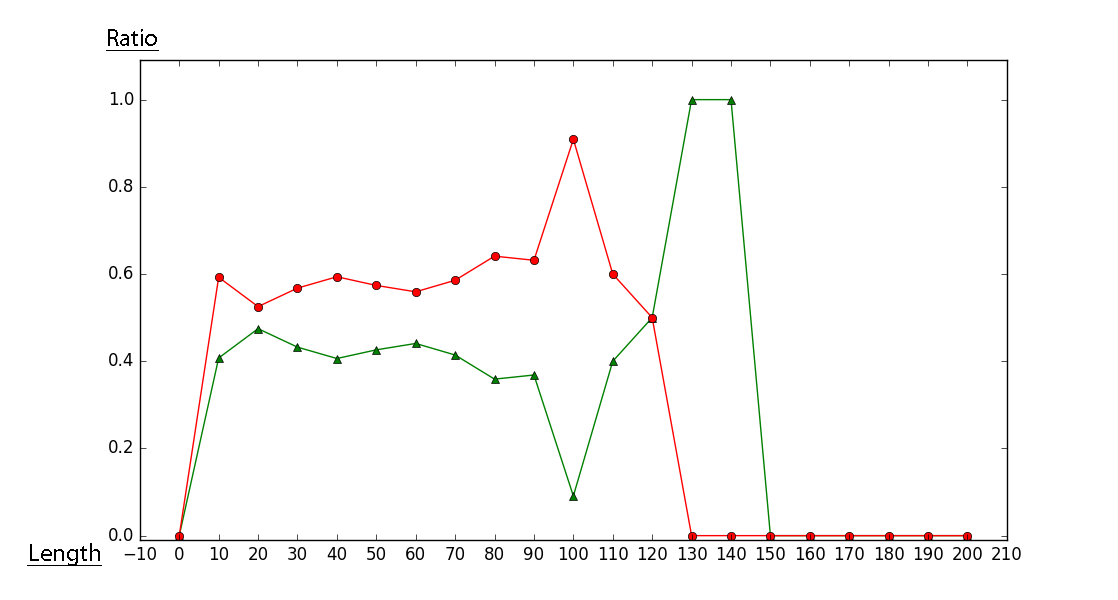
\includegraphics[width=.47\textwidth]{chapter4_experiments/images/length_errors.png}
}
\subfigure[Distance between entities dependency]{
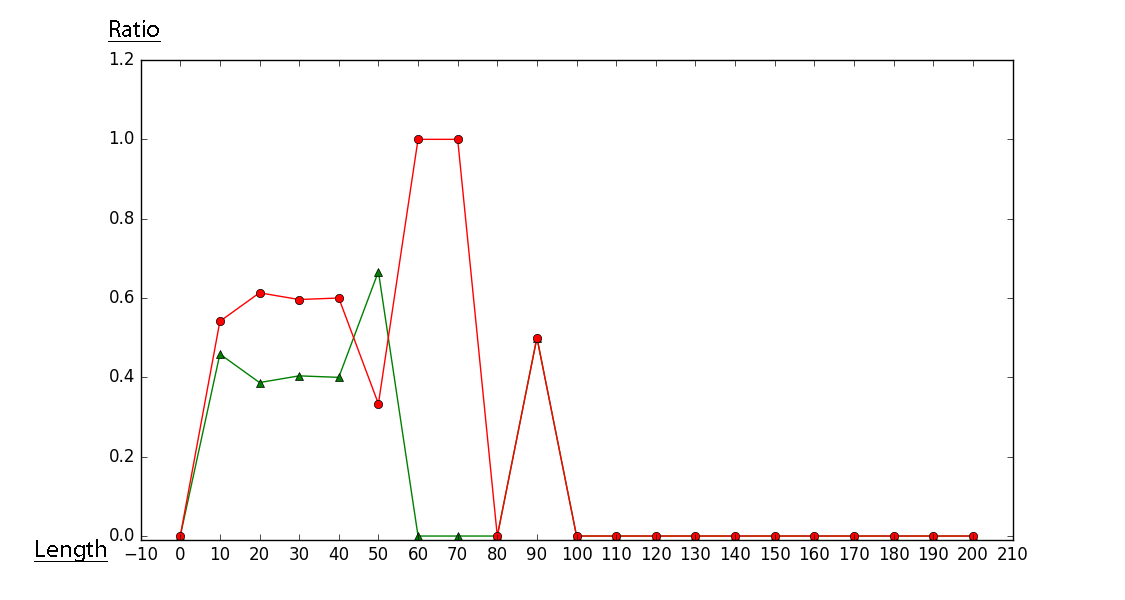
\includegraphics[width=.47\textwidth]{chapter4_experiments/images/betw_ent_errors.png}
}
\caption[Correlation of amount of correct and wrong answers with sentence length and distance between entities]{Dependency of the number of correct answers (green) and wrong answers (red) normalised by the overall amount of examples of specific length or with specific distance between entities correspondingly on the input sentence length and on the distance between entities.}
\label{fig:dist-depend}
\end{figure}

\paragraph{Representative trigrams}
If one takes a look at representative trigrams for the model trained on the distant dataset, mixed with 
supervised data and united in bags, several interesting observations can be made.
For example for relation ''per:spouse'', while supervised dataset obtained:

\textit{king george iii, his second wife, married gene raymond, wife melanie griffith, wife of actor, wife henrietta maria, husband jeff richmond, wife kimberly williams-paisley, wife of president}

newly trained model was able to obtain more general trigrams, such as:

\textit{wife of the, husband the, wife the, wife lee radziwill, wife of president, married yesterday to, wife of senator, wife of prime}

And the similar situation can be observed for several other relations. For example, 
''per:cities-of-residence'' becomes less unbiased in a sense of taking into account more cities, 
than it is in the training set.

\paragraph{Active learning}
\label{par:active-learn}
Even more interesting is an idea of exploiting representative trigrams as a tool for improving dataset. Thus, a look into 
representative trigrams obtained for the distantly supervised network can reveal some learned aspects that 
do not make sense from the human point of view. For example, for the relation ''org:founded-by'' found trigrams 
\textit{open society institute, fox broadcasting company, ethical treatment of, jack daniel's} seem to be 
not really representative. Same for the relation ''per:alternate-names'' a trigram \textit{mimi smith}. If these 
non representative trigrams are found in a sentence from the training dataset, the sentence might be 
filtered out, so the network will not learn the trigram anymore. A small experiment with two aforementioned 
relations showed improvement in scores. So, for ''org:founded-by'' Precision grew from 54.05 to 70 and 
Recall from 25 to 26.25. For ''per:alternate-names'' Precision improved from 33.33 to 38.24 and Recall 
from 21.74 to 28.26. This is a possibility to further improve Distant Supervision by application of Active Learning and iterative
transformations of the training dataset.
 

